\documentclass{report}

\usepackage{amsmath,amssymb}
\usepackage{graphicx}
\usepackage{enumitem}
\usepackage[total={6in,8in}]{geometry}
\usepackage{multicol}

\newcommand{\sol}{\textbf{Solution:}}
\newcommand{\proof}{\textbf{Proof:}}
\newcommand\perm[2][^n]{\prescript{#1\mkern-2.5mu}{}P_{#2}}
\newcommand\permtwo[2][^n]{{}_{#1}P_{#2}}
\newcommand\comb[2][^n]{{}_{#1}C_{#2}}
\newcommand\combtwo[2][^n]{\prescript{#1\mkern-2.5mu}{}C_{#2}}

\allowdisplaybreaks
\begin{document}
\begin{enumerate}[leftmargin=*]
    \item \begin{enumerate}
              \item Given that $h(x)=\dfrac{27}{4+x}, x \neq-4$, find the value of
                    \begin{enumerate}
                        \item $h^2(-1)$,

                              \sol{}
                              \begin{align*}
                                  h(-1)   & = \dfrac{27}{4+(-1)} \\
                                          & = \dfrac{27}{3}      \\
                                          & = 9                  \\
                                  h^2(-1) & = h(h(-1))           \\
                                          & = h(9)               \\
                                          & = \dfrac{27}{4+9}    \\
                                          & = \dfrac{27}{13}
                              \end{align*}

                        \item $h^{-1}(3)$.

                              \sol{}

                              Let $y = h^{-1}(x)$, then $x = h(y)$.
                              \begin{align*}
                                  x         & = \dfrac{27}{4+y}    \\
                                  4x+x y    & = 27                 \\
                                  x y       & = 27-4x              \\
                                  y         & = \dfrac{27-4x}{x}   \\
                                  h^{-1}(x) & = \dfrac{27-4x}{x}   \\
                                  h^{-1}(3) & = \dfrac{27-4(3)}{3} \\
                                            & = \dfrac{27-12}{3}   \\
                                            & = 5
                              \end{align*}
                    \end{enumerate}

              \item Given the functions $f g(x)=6 x-9$ and $g(x)=3 x+2$, find $f(x)$.

                    \sol{}

                    Let $y = g(x) = 3x + 2$, then $x = \dfrac{y-2}{3}$.
                    \begin{align*}
                        f(y) & = 6\left(\dfrac{y-2}{3}\right) - 9 \\
                             & = 2(y-2) - 9                       \\
                             & = 2y - 4 - 9                       \\
                             & = 2y - 13                          \\
                        f(x) & = 2x - 13
                    \end{align*}
          \end{enumerate}

    \item \begin{enumerate}
              \item Given that one of the roots of the quadratic equation $2 x^2-6 x+k=0$ is three
                    times the other root, find the value of $k$.

                    \sol{}

                    Let the roots be $p$ and $3p$, then
                    \begin{align*}
                        p+3p                              & = \dfrac{6}{2}  \\
                        4p                                & = 3             \\
                        p                                 & = \dfrac{3}{4}  \\
                        3p                                & = \dfrac{9}{4}  \\
                        (x-p)(x-3p)                       & = 0             \\
                        (x-\dfrac{3}{4})(x-\dfrac{9}{4})  & = 0             \\
                        x^2-\dfrac{12}{4}x+\dfrac{27}{16} & = 0             \\
                        2 x^2-6 x+\dfrac{27}{8}           & = 0             \\
                        k                                 & = \dfrac{27}{8}
                    \end{align*}

              \item Given the quadratic function $h(x)=x^2-12 x+3 p$, where $p$ is a constant.
                    \begin{enumerate}
                        \item Express $h(x)$ in the form $h(x)=(x+m)^2+n$, such that $m$ and $n$ are
                              constants.

                              \sol{}
                              \begin{align*}
                                  h(x) & = x^2-12 x+3 p         \\
                                       & = (x^2-12 x+36)-36+3 p \\
                                       & = (x-6)^2+3 p-36
                              \end{align*}

                        \item Given that the minimum value of $h(x)$ is -15 , find the value of $p$.

                              \sol{}
                              \begin{align*}
                                  h(x) & = (x-6)^2+3 p-36 \\
                                  -15  & = 3 p-36         \\
                                  3 p  & = 36-15          \\
                                  3 p  & = 21             \\
                                  p    & = 7
                              \end{align*}
                    \end{enumerate}
          \end{enumerate}

    \item \begin{enumerate}
              \item Find the range of values of $x$ for $6 x^2 \geqslant 3-7 x$.

                    \sol{}
                    \begin{align*}
                        6 x^2                                       & \geqslant 3-7 x                           \\
                        6 x^2+7 x-3                                 & \geqslant 0                               \\
                        (3 x-1)(2 x+3)                              & \geqslant 0                               \\
                        x              \geqslant \dfrac{1}{3} \quad & \text{or} \quad x \leqslant -\dfrac{3}{2}
                    \end{align*}

              \item Sketch the graph of $y=\left|x^2-4\right|$ for $-3 \leqslant x \leqslant 3$.

                    \sol{}

                    Lazy to draw the graph. =)

          \end{enumerate}

    \item Solve the following equations:
          \begin{enumerate}
              \item $8^{\log _2 u}=125$

                    \sol{}
                    \begin{align*}
                        8^{\log _2 u}     & = 125         \\
                        (2^3)^{\log _2 u} & = 5^3         \\
                        2^{3 \log _2 u}   & = 5^3         \\
                        3 \log _2 u       & = 3 \log _2 5 \\
                        \log _2 u         & = \log _2 5   \\
                        u                 & = 5
                    \end{align*}

              \item $\log _{81}\left[\log _2(3 x-10)\right]=\dfrac{1}{4}$

                    \sol{}
                    \begin{align*}
                        \log _{81}\left[\log _2(3 x-10)\right] & = \dfrac{1}{4}    \\
                        81^{\frac{1}{4}}                       & = \log _2(3 x-10) \\
                        \log_2(3 x-10)                         & = 3               \\
                        3x-10                                  & = 2^3             \\
                        3x                                     & = 8+10            \\
                        x                                      & = 6
                    \end{align*}
          \end{enumerate}

    \item In Diagram $1, A B C$ is an isosceles triangle such that $A B=A C=16
              \mathrm{~cm}$. $D B E$ is a sector with centre $B$ and a radius of $14
              \mathrm{~cm}$.

          \begin{center}
              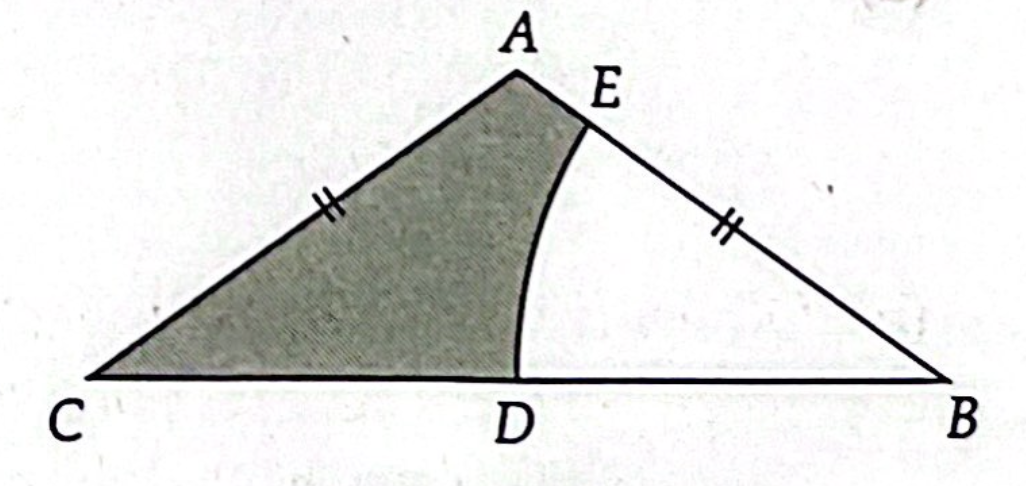
\includegraphics[width=0.4\textwidth]{./assets/p1.5.png}
          \end{center}

          Given that $A$ is vertically above $D$, find
          \begin{enumerate}
              \item $\angle D B E$, in radians,

                    \sol{}
                    \begin{align*}
                        \cos \angle D B E & = \dfrac{DB}{AB} = \dfrac{14}{16} = \dfrac{7}{8} \\
                        \angle D B E      & = \cos^{-1}\left(\dfrac{7}{8}\right)             \\
                                          & = 0.5054 \text{ rad}
                    \end{align*}

              \item the area, in $\mathrm{cm}^2$, of the shaded region.

                    \sol{}
                    \begin{align*}
                        \dfrac{AD}{AB}                 & = \sin 0.5054                            \\
                        AD                             & = 16 \sin 0.5054                         \\
                                                       & = 7.746 \mathrm{~cm}                     \\
                        \text{Area of $\triangle ABC$} & = \dfrac{1}{2} \times 28 \times 7.746    \\
                                                       & = 108.4435\mathrm{~cm}^2                 \\
                        \text{Area of sector $DBE$}    & = \dfrac{1}{2} \times 14^2 \times 0.5054 \\
                                                       & = 49.52 \mathrm{~cm}^2                   \\
                        \text{Area of shaded region}   & = 108.4435-49.52                         \\
                                                       & = 58.92\mathrm{~cm}^2
                    \end{align*}
          \end{enumerate}

    \item \begin{enumerate}
              \item Sketch the graph of $y=4 \sin \dfrac{3 x}{2}$ for $0 \leqslant x \leqslant
                        \pi$.

                    \sol{}

                    Lazy to draw the graph. =)

              \item Solve the equation $2 \sin 2 x=\cos x$ for $0^{\circ} \leqslant x \leqslant
                        360^{\circ}$.

                    \sol{}
                    \begin{align*}
                        2 \sin 2 x                                 & = \cos x                                                     \\
                        4 \sin x \cos x                            & = \cos x                                                     \\
                        4 \sin x\cos x - \cos x                    & = 0                                                          \\
                        \cos x(4 \sin x - 1)                       & = 0                                                          \\
                        \cos x = 0                                 & \text{ or } \sin x = \dfrac{1}{4}                            \\
                        x = 90^{\circ} \text{ or } x = 270^{\circ} & \text{ or } x = 14.48^{\circ} \text{ or } x = 165.52^{\circ}
                    \end{align*}
          \end{enumerate}

    \item Diagram 2 shows part of the line of best fit obtained by plotting $\log _2 y$
          against $\log _2 x$.

          \begin{center}
              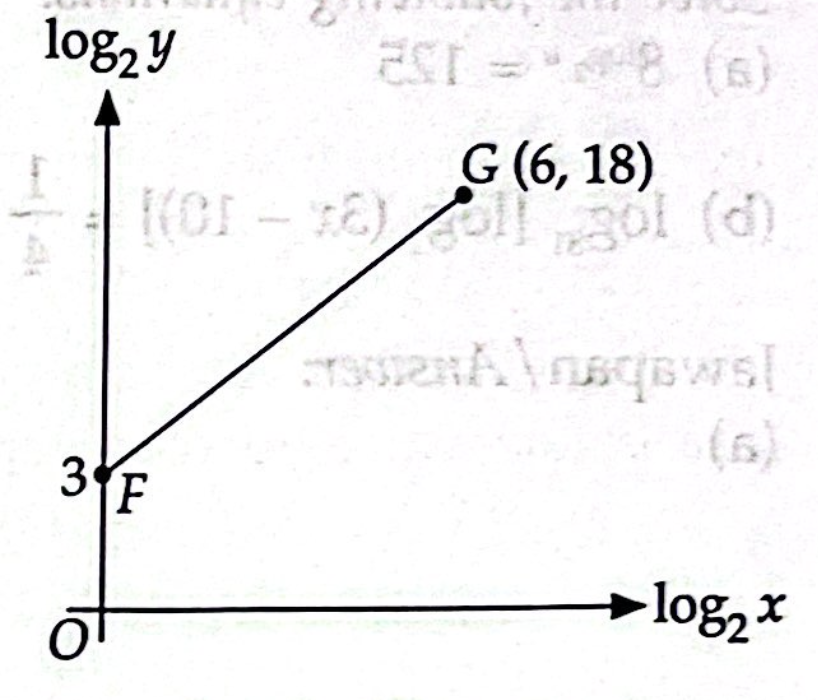
\includegraphics[width=0.4\textwidth]{./assets/p1.7.png}
          \end{center}

          Given that $y=m x^n$, such that $m$ and $n$ are constants, find
          \begin{enumerate}
              \item the value of $m$ and of $n$,

                    \sol{}
                    \begin{align*}
                        \text{Gradient}         & = \dfrac{18 - 3}{6 - 0} = \dfrac{5}{2} \\
                        \text{Intercept}        & = 3                                    \\
                        \log_2 y                & = \dfrac{5}{2} \log_2 x + 3            \\
                        2\log_2 y               & = 5\log_2 x + 6                        \\
                        \log_2 y^2              & = \log_2 x^5 + 6                       \\
                        \log_2 y^2       - \log_2 x^5 = 6                                \\
                        \log_2 \dfrac{y^2}{x^5} & = 6                                    \\
                        \dfrac{y^2}{x^5}        & = 64                                   \\
                        y^2                     & = 64 x^5                               \\
                        y                       & = 8 x^{\frac{5}{2}}
                    \end{align*}
                    $\therefore$ $m = 8$ and $n = \dfrac{5}{2}$.

              \item the value of $y$ when $x=4$.

                    \sol{}
                    \begin{align*}
                        y & = 8 x^{\frac{5}{2}}        \\
                          & = 8 \times 4^{\frac{5}{2}} \\
                          & = 8 \times 32              \\
                          & = 256
                    \end{align*}
          \end{enumerate}

    \item \begin{enumerate}
              \item Given that $y=x(3 x+1)(2 x-3)$, find $\dfrac{d y}{d x}$.

                    \sol{}
                    \begin{align*}
                        y                & = x(3 x+1)(2 x-3)    \\
                                         & = x(6 x^2-9 x+2 x-3) \\
                                         & = 6 x^3-7 x^2-3 x    \\
                        \dfrac{d y}{d x} & = 18 x^2-14 x-3
                    \end{align*}

                    \newpage
              \item The volume of a spherical balloon that is leaking decreases at a rate of
                    $\dfrac{\pi}{2} \mathrm{~cm}^3 \mathrm{~s}^{-1}$. Find the rate of change of
                    its radius when the radius is $1 \mathrm{~cm}$.

                    \sol{}
                    \begin{align*}
                        V                & = \dfrac{4}{3} \pi r^3                            \\
                        \dfrac{d V}{d r} & = 4 \pi r^2                                       \\
                        \dfrac{dV}{dt}   & = -\dfrac{\pi}{2}                                 \\
                        \dfrac{dr}{dt}   & = \dfrac{dr}{dV} \times \dfrac{dV}{dt}            \\
                                         & = \dfrac{1}{4 \pi r^2} \times -\dfrac{\pi}{2}     \\
                                         & = -\dfrac{1}{8 r^2} \mathrm{~cm} \mathrm{~s}^{-1}
                    \end{align*}
                    When $r = 1 \mathrm{~cm}$,
                    \begin{align*}
                        \dfrac{dr}{dt} & = -\dfrac{1}{8(1)^2}                          \\
                                       & = -\dfrac{1}{8} \mathrm{~cm} \mathrm{~s}^{-1}
                    \end{align*}
                    $\therefore$ the rate of change of its radius is $-\dfrac{1}{8} \mathrm{~cm}
                        \mathrm{~s}^{-1}$ when the radius is $1 \mathrm{~cm}$.
          \end{enumerate}

    \item Diagram 3 shows a rod $F H$ of length $1.5 \mathrm{~cm}$ is leaning against a
          wall at point $F$ and touches the floor at point $H$. Point $G$ divides the rod
          in the ratio $1: 2$.
          \begin{center}
              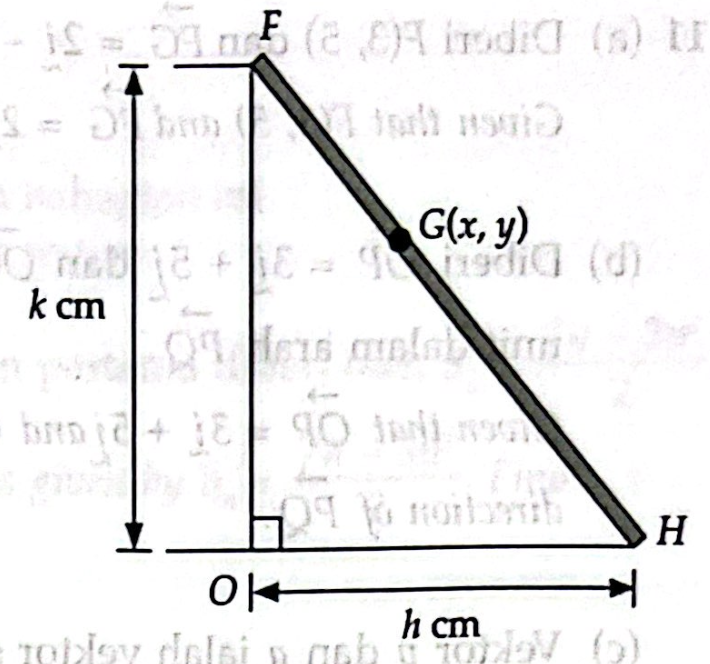
\includegraphics[width=0.4\textwidth]{./assets/p1.9.png}
          \end{center}

          If the rod is sliding down, show that the equation of locus of the moving point
          $G$ is $4 x^2+y^2=1$.

          \sol{}
          \begin{align*}
              k^2 + h^2 & = 1.5^2             \\
              k^2 + h^2 & = 2.25\ \cdots\ (1)
          \end{align*}

          Let the coordinates of F be $(0, k)$ and the coordinates of H be $(h, 0)$.
          \begin{align*}
              x & = \dfrac{2(0) + h}{3} = \dfrac{h}{3}  \\
              h & = 3x\ \cdots\ (2)                     \\
              y & = \dfrac{2(k) + 0}{3} = \dfrac{2k}{3} \\
              k & = \dfrac{3y}{2}\ \cdots\ (3)
          \end{align*}
          Substituting $(2)$ and $(3)$ into $(1)$,
          \begin{align*}
              \left(3x\right)^2 + \left(\dfrac{3y}{2}\right)^2 & = 2.25 \\
              9x^2 + \dfrac{9y^2}{4}                           & = 2.25 \\
              36x^2 + 9y^2                                     & = 9    \\
              4x^2 + y^2                                       & = 1
          \end{align*}

    \item Diagram 4 shows part of a plan of three straight roads.
          \begin{center}
              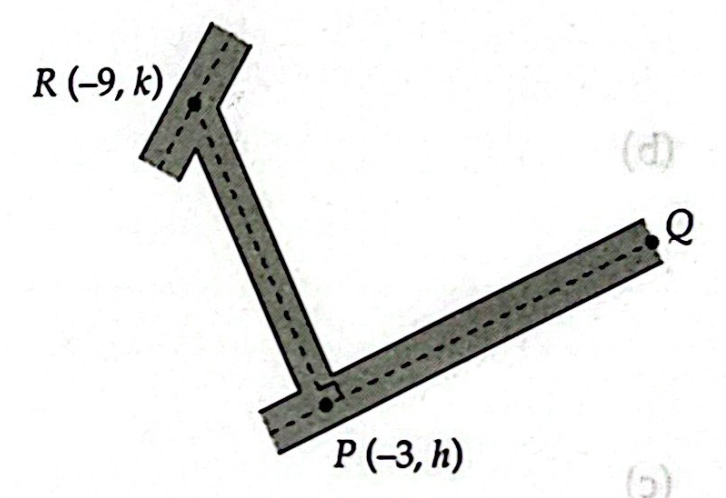
\includegraphics[width=0.4\textwidth]{./assets/p1.10.png}
          \end{center}

          The straight road $P Q$ is represented by the equation $2 y=x-7$.

          Find
          \begin{enumerate}
              \item the value of $h$,

                    \sol{}
                    When $x = -3$,
                    \begin{align*}
                        2y            & = -3 - 7 \\
                        2y            & = -10    \\
                        y             & = -5     \\
                        \therefore\ h & = -5
                    \end{align*}

              \item the equation of the straight road $P R$,

                    \sol{}
                    The gradient of $P Q$ is $\dfrac{1}{2}$, therefore the gradient of $P R$ is $-2$.

                    Let the equation of $P R$ is
                    \begin{align*}
                        y + 5 & = -2(x + 3) \\
                        y     & = -2x - 11
                    \end{align*}

              \item the value of $k$. When $x = -9$,
                    \begin{align*}
                        y             & = -2(-9) - 11 \\
                                      & = 7           \\
                        \therefore\ k & = 7
                    \end{align*}
          \end{enumerate}

    \item \begin{enumerate}
              \item Given that $F(3,5)$ and $\overrightarrow{F G}=2 \vec{\imath}-8 \vec{\jmath}$,
                    find the coordinates of $G$.

                    \sol{}
                    \begin{align*}
                        \overrightarrow{FG} & = \overrightarrow{OG} - \overrightarrow{OF}                     \\
                        \overrightarrow{OG} & = \overrightarrow{OF} + \overrightarrow{FG}                     \\
                                            & = 3\vec{\imath} + 5\vec{\jmath} + 2\vec{\imath} - 8\vec{\jmath} \\
                                            & = 5\vec{\imath} - 3\vec{\jmath}
                    \end{align*}
                    Therefore, the coordinates of $G$ are $(5, -3)$.

              \item Given that $\overrightarrow{O P}=3 \vec{\imath}+5 \vec{\jmath}$ and
                    $\overrightarrow{O Q}=7 \vec{\imath}-6 \vec{\jmath}$, such that $O$ is the
                    origin, find the unit vector in the direction of $\overrightarrow{P Q}$.

                    \sol{}
                    \begin{align*}
                        \overrightarrow{PQ}                         & = \overrightarrow{OQ} - \overrightarrow{OP}                     \\
                                                                    & = 7\vec{\imath} - 6\vec{\jmath} - 3\vec{\imath} - 5\vec{\jmath} \\
                                                                    & = 4\vec{\imath} - 11\vec{\jmath}                                \\
                        \text{Magnitude of $\overrightarrow{PQ}$}   & = \sqrt{4^2 + (-11)^2}                                          \\
                                                                    & = \sqrt{16 + 121}                                               \\
                                                                    & = \sqrt{137}                                                    \\
                        \text{Unit vector of $\overrightarrow{PQ}$} & = \dfrac{\overrightarrow{PQ}}{|\overrightarrow{PQ}|}            \\
                                                                    & = \dfrac{4\vec{\imath} - 11\vec{\jmath}}{\sqrt{137}}
                    \end{align*}

              \item Vectors $\vec{p}$ and $\vec{q}$ are parallel vectors. It is given that $|3 a-b|
                        \vec{p}=4 \vec{q}$, where $a$ and $b$ are constants. Express $a$ in terms of
                    $b$.

                    \sol{}

                    Skipped cuz very sus.
          \end{enumerate}

          \newpage
    \item Given that $y=\dfrac{48}{x^4}$
          \begin{enumerate}
              \item find the value of $\dfrac{d y}{d x}$ when $x=2$,

                    \sol{}
                    \begin{align*}
                        y                & = 48x^{-4}   \\
                        \dfrac{d y}{d x} & = -192x^{-5}
                    \end{align*}
                    When $x = 2$,
                    \begin{align*}
                        \dfrac{d y}{d x} & = -192(2)^{-5}              \\
                                         & = -192 \times \dfrac{1}{32} \\
                                         & = -6
                    \end{align*}

              \item without using calculator, find the approximate value of $\dfrac{48}{1.996^4}$.

                    \sol{}
                    \begin{align*}
                        \dfrac{\delta y}{\delta x} & \approx \dfrac{dy}{dx}                 \\
                        \delta y                   & \approx \dfrac{dy}{dx} \times \delta x
                    \end{align*}
                    When $x = 2$, $\delta x = -0.004$, $y = \dfrac{48}{2^4} = 3$.
                    \begin{align*}
                        \delta y     & \approx -6 \times -0.004 \\
                                     & = 0.024                  \\
                        \therefore y & \approx 3 + 0.024        \\
                                     & = 3.024
                    \end{align*}
          \end{enumerate}

    \item \begin{enumerate}
              \item In an arithmetic progression, the sum of the first $n$ terms is given by
                    $S_n=\dfrac{7 n-3 n^2}{2}$. Find
                    \begin{enumerate}
                        \item the $9^{\text {th }}$ term,

                              \sol{}
                              \begin{align*}
                                  T_9 & = S_9 - S_8                                           \\
                                      & = \dfrac{7(9) - 3(9)^2}{2} - \dfrac{7(8) - 3(8)^2}{2} \\
                                      & = \dfrac{63 - 243}{2} - \dfrac{56 - 192}{2}           \\
                                      & = -90 - (-68)                                         \\
                                      & = -22
                              \end{align*}

                              \newpage
                        \item the $n^{\text {th }}$ term.

                              \sol{}
                              \begin{align*}
                                  T_1 & = S_1                          \\
                                      & = \dfrac{7(1) - 3(1)^2}{2}     \\
                                      & = 2                            \\
                                  T_2 & = S_2 - S_1                    \\
                                      & = \dfrac{7(2) - 3(2)^2}{2} - 2 \\
                                      & = -1                           \\
                                  d   & = -1 - 2 = -3                  \\
                                  T_n & = 2 + (-3)(n-1)                \\
                                      & = 2 - 3n + 3                   \\
                                      & = 5 - 3n
                              \end{align*}
                    \end{enumerate}

              \item Given that $p, q, 72$ and 216 are the first four terms of a geometric
                    progression, find
                    \begin{enumerate}
                        \item the value of $p$ and of $q$,

                              \sol{}
                              \begin{align*}
                                  \dfrac{72}{q} & = \dfrac{216}{72} \\
                                  216q          & = 72^2            \\
                                  q             & =24               \\
                                  \\
                                  \dfrac{24}{p} & = \dfrac{72}{24}  \\
                                  72p           & = 24^2            \\
                                  p             & =8
                              \end{align*}

                        \item the sum of the $7^{\text {th }}$ term to the $9^{\text {th }}$ term. \sol{}
                              \begin{align*}
                                  a = 8, & \ r = 3                     \\
                                  S_n    & = \dfrac{8(3^n - 1)}{3 - 1} \\
                                         & = 4(3^n - 1)                \\
                                  S      & = S_9 - S_6                 \\
                                         & = 4(3^9 - 1) - 4(3^6 - 1)   \\
                                         & = 75816
                              \end{align*}
                    \end{enumerate}
          \end{enumerate}

          \newpage
    \item \begin{enumerate}
              \item Given that $\displaystyle\int_1^3 h(x) d x=m$, find in terms of $m$ for
                    \begin{enumerate}
                        \item  $\displaystyle\int_1^3 \dfrac{5 h(x)}{2} d x$,

                              \sol{}
                              \begin{align*}
                                  \int_1^3 \dfrac{5 h(x)}{2} d x & = \dfrac{5}{2} \int_1^3 h(x) d x \\
                                                                 & = \dfrac{5}{2} m
                              \end{align*}

                        \item  $\displaystyle\int_1^3[6 x+2 h(x)] d x$.

                              \sol{}
                              \begin{align*}
                                  \int_1^3[6 x+2 h(x)] d x & = \int_1^3 6 x d x + \int_1^3 2 h(x) d x          \\
                                                           & = 6 \int_1^3 x d x + 2 \int_1^3 h(x) d x          \\
                                                           & = 6 \left[\dfrac{x^2}{2}\right]_1^3 + 2m          \\
                                                           & = 6 \left[\dfrac{9}{2} - \dfrac{1}{2}\right] + 2m \\
                                                           & = 24 + 2m
                              \end{align*}
                    \end{enumerate}
              \item Diagram 5 shows a curve $y^2=\dfrac{16}{x}$.
                    \begin{center}
                        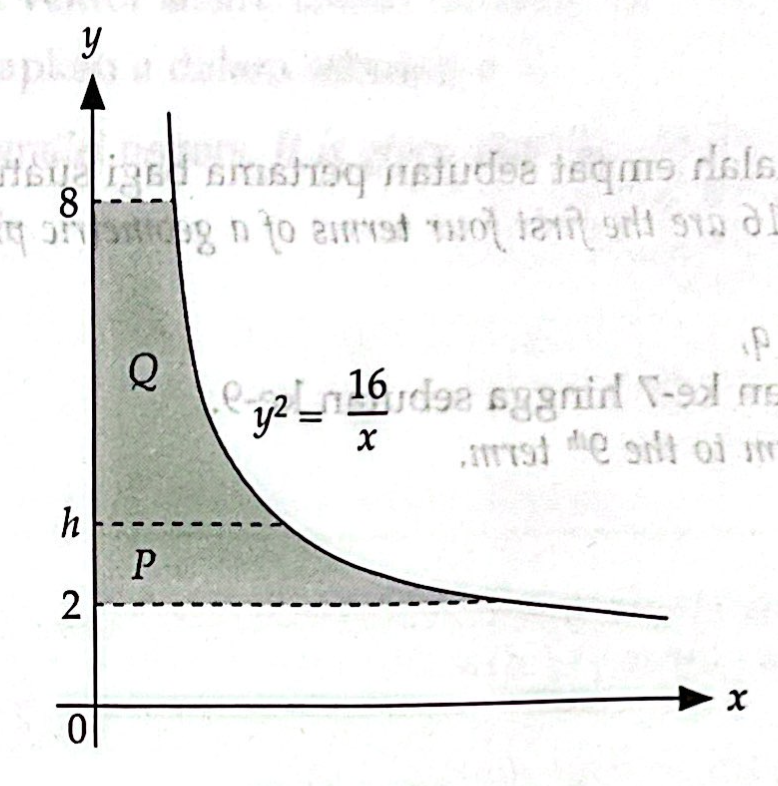
\includegraphics[scale=0.25]{assets/p1.14b.png}
                    \end{center}

                    Given that the area of the shaded region $P=$ area of the shaded region $Q$,
                    find the value of $h$.

                    \sol{}
                    \begin{align*}
                        y^2                             & = \dfrac{16}{x}                   \\
                        x                               & = \dfrac{16}{y^2}                 \\
                        \int_2^h \dfrac{16}{y^2} d y    & = \int_h^8 \dfrac{16}{y^2} d y    \\
                        \left[-\dfrac{16}{y}\right]_2^h & = \left[-\dfrac{16}{y}\right]_h^8 \\
                        -\dfrac{16}{h} + 8              & = -2 + \dfrac{16}{h}              \\
                        10                              & = \dfrac{32}{h}                   \\
                        h                               & = 3.2
                    \end{align*}
          \end{enumerate}

    \item \begin{enumerate}
              \item Five students are to be chosen from a group of four boys and six girls to
                    represent a school in a Mathematics quiz competition. Calculate the number of
                    teams that can be formed if each team consists of
                    \begin{enumerate}
                        \item one boy and four girls,

                              \sol{}

                              First, choose 1 boy from 4 boys, there are $\comb[4]{1}$ ways to do this.

                              Then, choose 4 girls from 6 girls, there are $\comb[6]{4}$ ways to do this.

                              Hence, the number of teams that can be formed is $\comb[4]{1} \times
                                  \comb[6]{4} = 4 \times 15 = 60$.

                        \item at least two boys.

                              \sol{}

                              The number of teams that can be formed is
                              \begin{align*}
                                  \comb[10]{5} - \comb[4]{0} \times \comb[6]{5} - \comb[4]{1} \times \comb[6]{4} & = 252 - 6 - 60 \\
                                                                                                                 & = 186
                              \end{align*}
                    \end{enumerate}

              \item The masses of several bags of flour, in $\mathrm{kg}$, are normally distributed
                    with a mean of $\mu$ and a standard deviation of $\sigma$. It is given that
                    $3.45 \%$ of bags of flour have masses more than $35 \mathrm{~kg}$ and $24.2
                        \%$ have masses less than $20 \mathrm{~kg}$. Find the the value of $\mu$ and of
                    $\sigma$.

                    \sol{}

                    Let $X$ be the mass of a bag of flour, then $Z \sim \dfrac{X - \mu}{\sigma}$ is
                    a standard normal distribution.
                    \begin{align*}
                        P(X > 35)                                  & = 0.0345                               \\
                        P\left(Z > \dfrac{35 - \mu}{\sigma}\right) & = 0.0345                               \\
                        \dfrac{35 - \mu}{\sigma}                   & = 1.82                                 \\
                        \sigma                                     & = \dfrac{35 - \mu}{1.82}\ \cdots\ (1)  \\
                        \\
                        P(X < 20)                                  & = 0.242                                \\
                        P\left(Z < \dfrac{20 - \mu}{\sigma}\right) & = 0.242                                \\
                        P\left(Z > \dfrac{\mu - 20}{\sigma}\right) & = 0.242                                \\
                        \dfrac{\mu - 20}{\sigma}                   & = 0.70                                 \\
                        \sigma                                     & = \dfrac{\mu - 20}{0.70} \ \cdots\ (2)
                    \end{align*}
                    Equating $(1)$ and $(2)$,
                    \begin{align*}
                        \dfrac{35 - \mu}{1.82} & = \dfrac{\mu - 20}{0.70}                  \\
                        35 - \mu               & = 1.82\left(\dfrac{\mu - 20}{0.70}\right) \\
                        35 - \mu               & = 2.6(\mu - 20)                           \\
                        35 - \mu               & = 2.6\mu - 52                             \\
                        52 + 35                & = 2.6\mu + \mu                            \\
                        87                     & = 3.6\mu                                  \\
                        \mu                    & = 24.17\mathrm{~kg}
                    \end{align*}
                    Substituting $\mu = 24.17$ into $(1)$,
                    \begin{align*}
                        \sigma & = \dfrac{35 - \dfrac{87}{3.6}}{1.82} \\
                               & = 5.952\mathrm{~kg}
                    \end{align*}
                    Therefore, $\mu = 24.17\mathrm{~kg}$ and $\sigma = 5.952\mathrm{~kg}$.
          \end{enumerate}
\end{enumerate}
\end{document}